\section{Introduction}
\label{sec:introduction}
% Unnumbered inset: the approved mechanism overview remains Figure 1.
\begin{wrapfigure}[24]{r}{2.70in}
\vspace{-3.5\baselineskip}
\centering
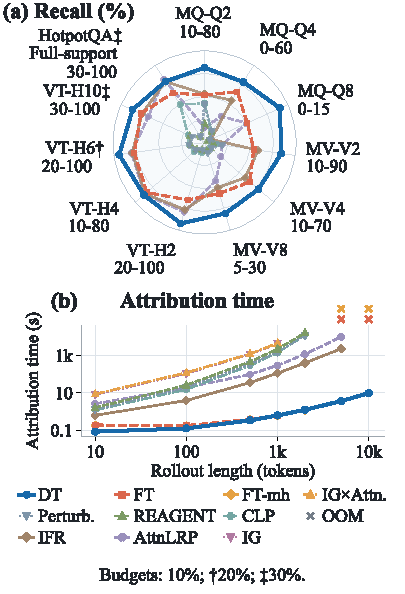
\includegraphics[width=2.70in]{results/figures/deltatrace-recall-time.pdf}
\vspace{-\intextsep}
\end{wrapfigure}


Input attribution assigns scores to the words in a prompt to explain a model's response. A reasoning response depends on both the information available and the computations that select and combine it \citep{ferrando2024information}. Figure~\ref{fig:overview}(d) shows a passage containing a playwright, William Shakespeare, and a composer, William Walton. The names supply candidate answers, and the phrase ``the author of the play'' specifies which role to use. An explanation should follow both the supplied content and the control that directs its use. It should also distinguish words that support the response from words that oppose it.

We ask how replacing selected prompt tokens would change the model's score for a chosen response span. The reference replaces these source tokens with end-of-sequence (EOS) tokens at the same positions. Both executions score the same target span using the fixed response prefix. The target can be an answer span or the complete reasoning and answer. We assign each source token a signed share of the resulting log-probability difference, so the contributions add across words or passages.

\begin{figure}[t]
\centering
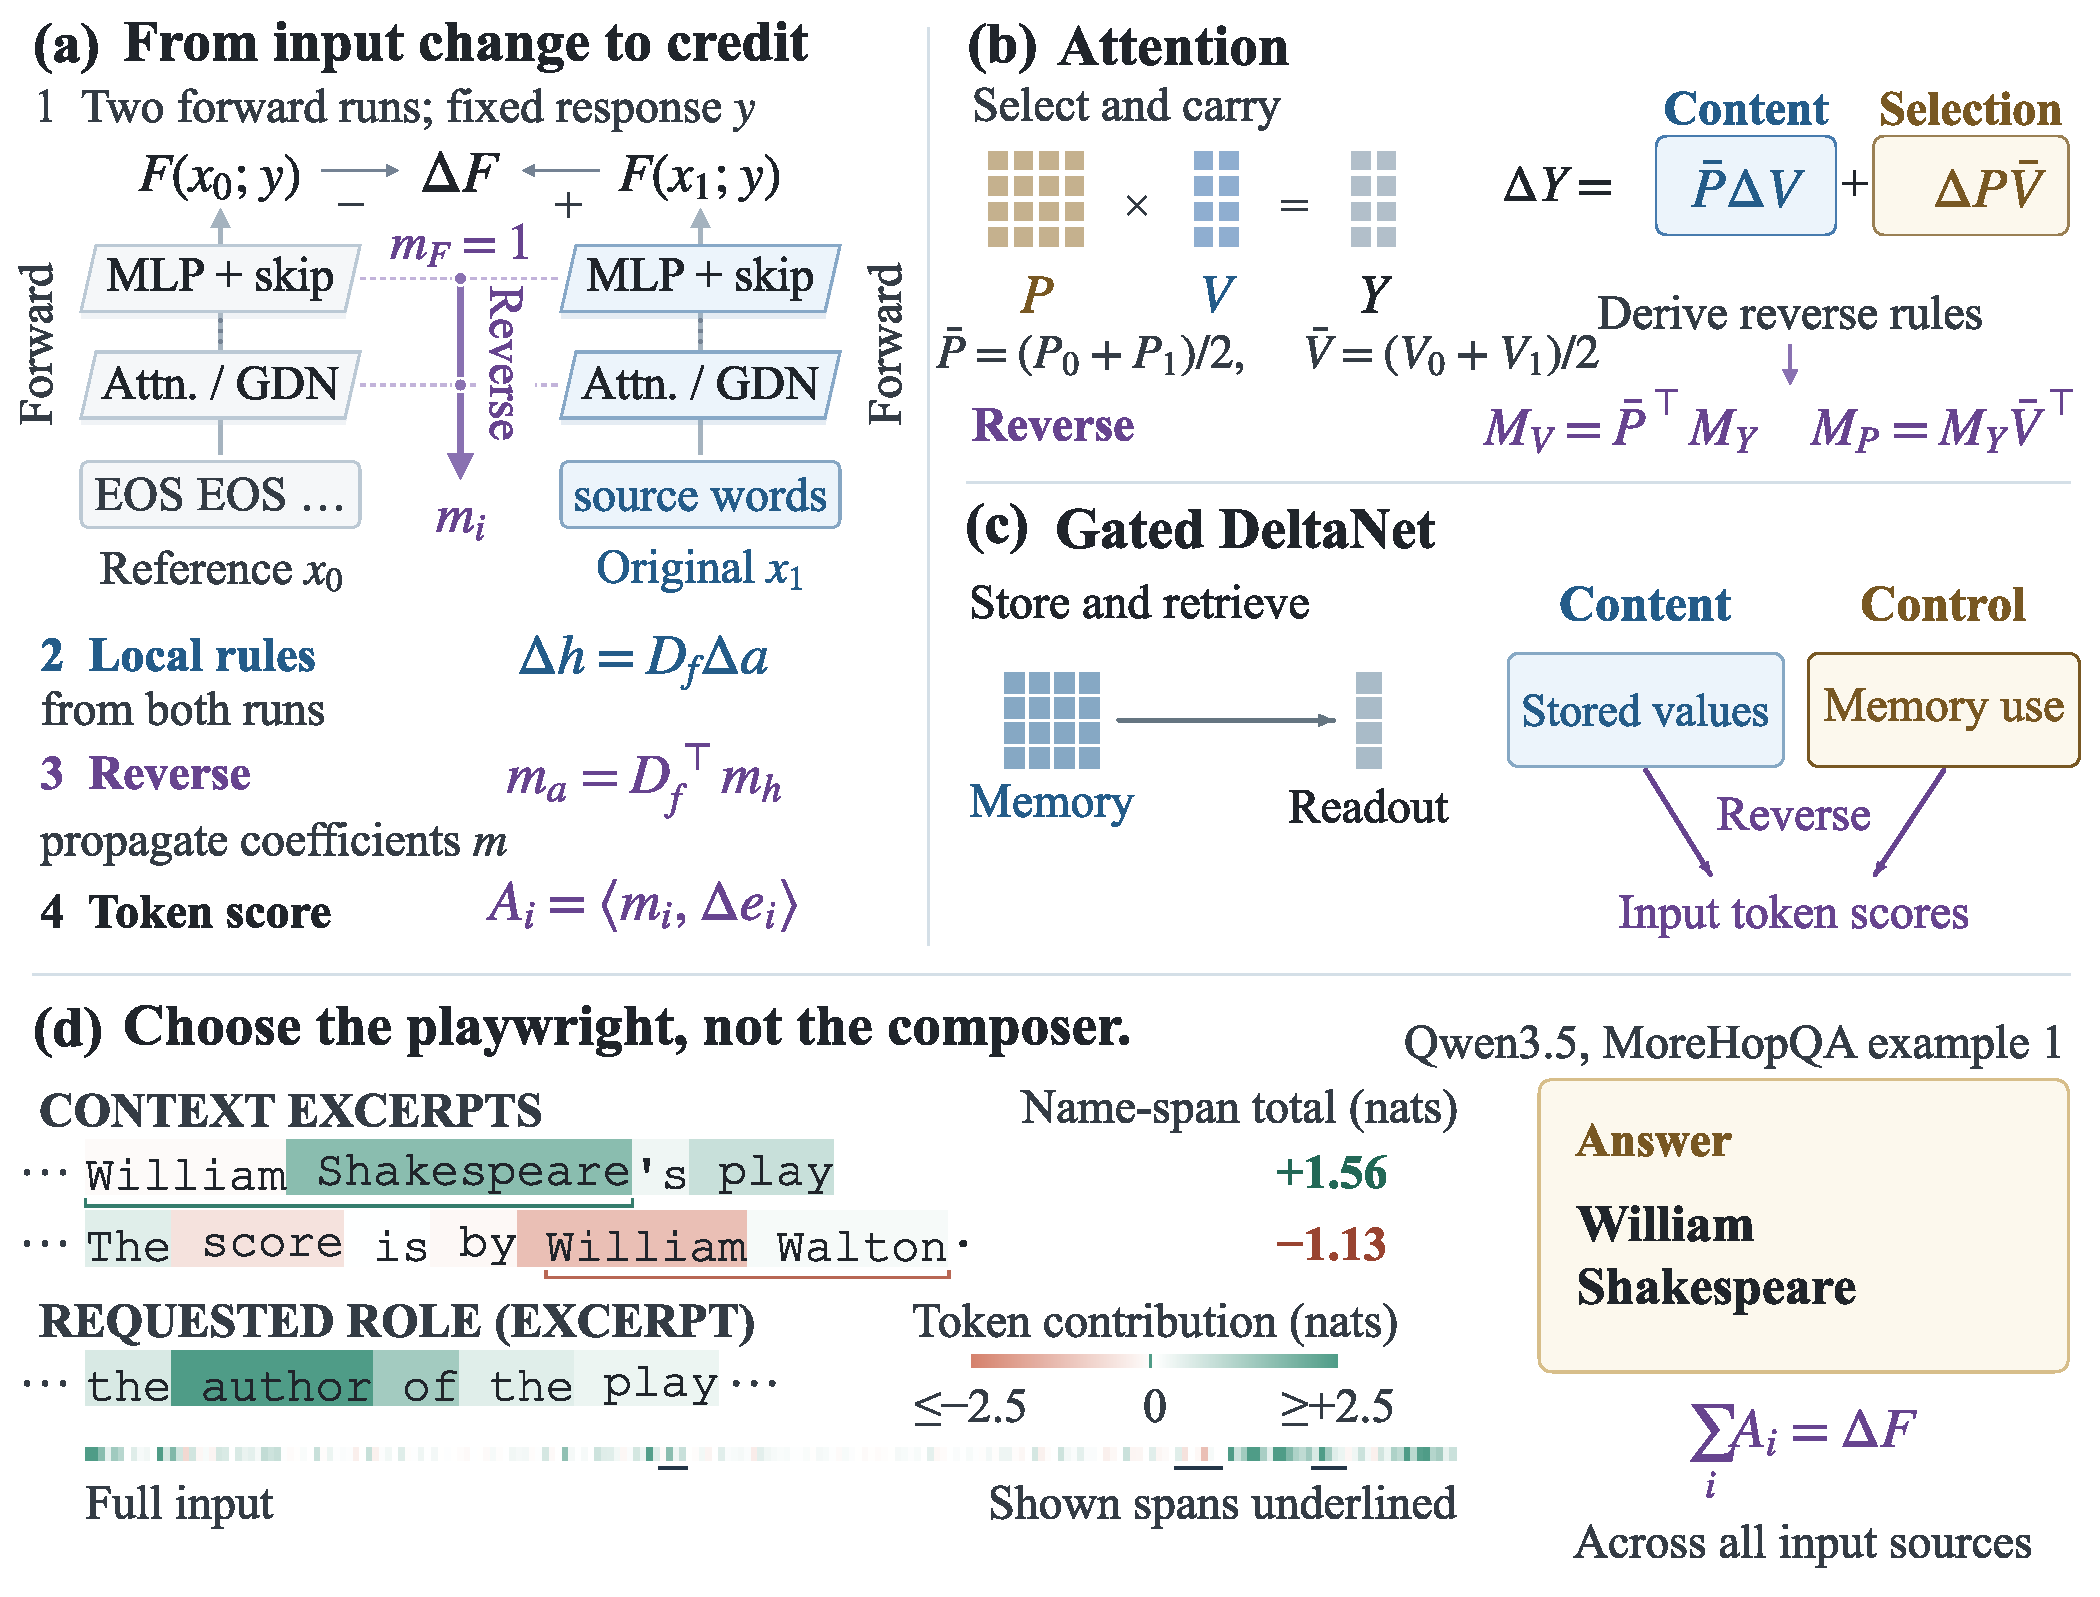
\includegraphics[width=\linewidth]{figures/generated/deltatrace-mechanism.pdf}

\caption{\textbf{DeltaTrace follows content and control.} (a) Gray arrows show the original and reference forward runs. The purple reverse pass propagates coefficients backward to compute token scores that sum to their score difference $\Delta F$. (b) Attention assigns credit through values and selection. Bars denote averages of the two runs. (c) GDN assigns credit through stored values and the operations controlling their use. Both paths continue to input token scores. (d) Qwen3.5 assigns positive scores to the playwright's name and negative scores to the composer's. Colors saturate at $\pm2.5$ nats, and annotations sum the marked names. Ellipses omit text. The target includes the complete stored response and EOS.}
\label{fig:overview}
\end{figure}

Reference-based methods already assign prediction differences to inputs through integrated gradients or propagated activation differences \citep{sundararajan2017axiomatic,shrikumar2017deeplift}. Relevance propagation and representation decomposition trace how information moves through attention and recurrent states \citep{ali2022conservative,achtibat2024attnlrp,jafari2024mambalrp,modarressi2023decompx,pitorro2025latim}. FlashTrace follows source importance through multi-token responses \citep{pan2026flashtrace}. \dt{} provides analytic finite rules that allocate a complete response-score difference through attention selection and gated-memory updates.

The difficulty is that content and control change together. Changing a token can alter both its value vector and the attention weights that select it. Those weights compete because their sum is one. In gated memory, a new value changes a state assembled from earlier tokens, while keys, queries, and gates determine what is written, retained, and read \citep{yang2024gated}. Tracing only the transported content leaves these selection and memory decisions outside the explanation. Tracing both requires local rules that account for their joint changes and can be composed across the whole response.

\dt{} begins with two forward runs that supply the original and reference activations. Analytic rules use these pairs to replace each local Jacobian with a finite map. One reverse pass applies the transposed maps to coefficients, starting with $1$ at the response score. At the input, each coefficient vector is dotted with its embedding difference to obtain a token attribution score. These scores sum to the response-score difference.

The computation follows the same structure as accelerated attention. FlashAttention-style tiles process small blocks of token interactions \citep{dao2022flashattention}, and Flash Linear Attention (FLA) processes memory in consecutive chunks \citep{yang2024fla}. Accumulating coefficients within these blocks gives auxiliary storage linear in sequence length at fixed model dimensions and chunk size.

On Qwen3-8B retrieval and reasoning tasks, \dt{} achieves the lowest deletion-faithfulness scores on most tasks and the highest evidence recovery across the six needle-in-a-haystack tasks (Section~\ref{sec:evaluation}). Qwen3.5-9B measurements evaluate finite reverse propagation through attention and gated memory. Appendix~\ref{app:credit} discusses the connection between counterfactual return differences and policy advantages \citep{sutton1999policy,foerster2018counterfactual}.
